\section{Handskizzen}
\setauthor{Raffeiner Christine}

Aus den Erkenntnissen der Umfeldanalyse wurden in der ersten Instanz einfache Handskizzen (siehe Abb. \ref{fig:skizzen1} und \ref{fig:skizzen2}) für das Design angefertigt.
Bereits in den ersten Skizzen kristallisierten sich spezielle Ideen, wie zum Beispiel das Dashboard, heraus.

\begin{figure}[H]
    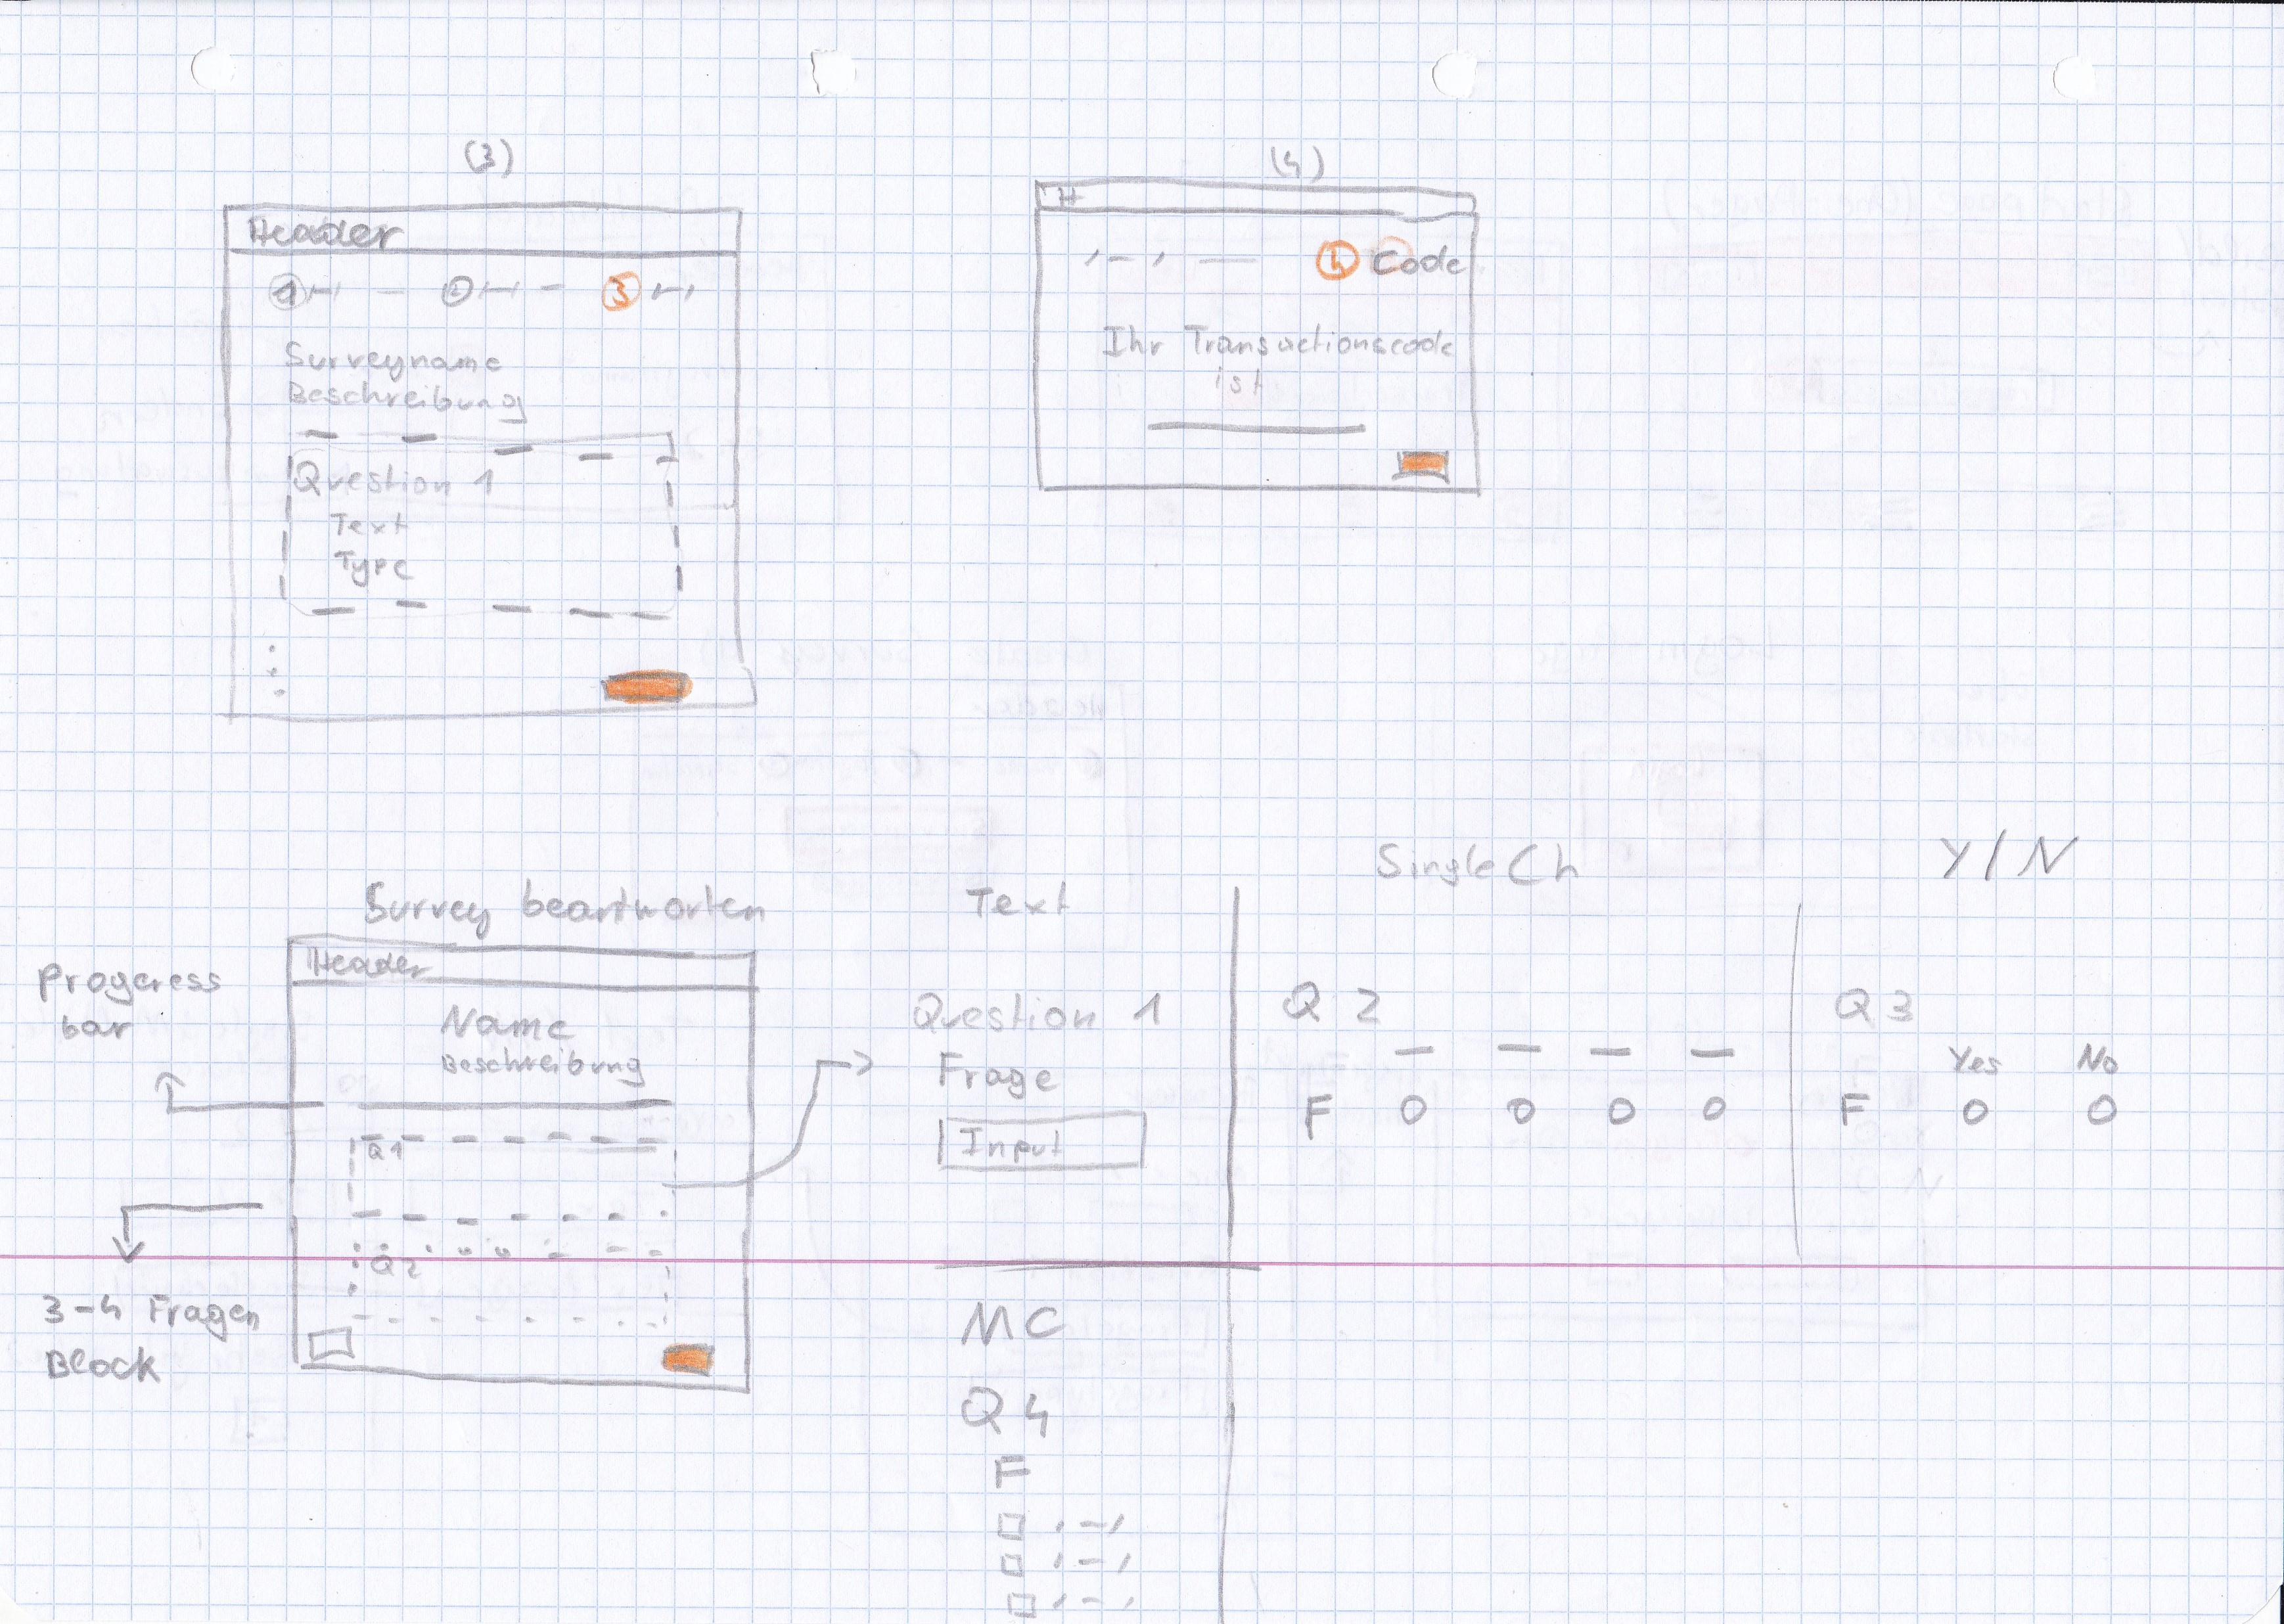
\includegraphics[width=1.0\textwidth]{pics/Handskizze.jpg}
    \centering
    \caption{Skizze Seite 1}
    \label{fig:skizzen1}
\end{figure}

\begin{figure}[H]
    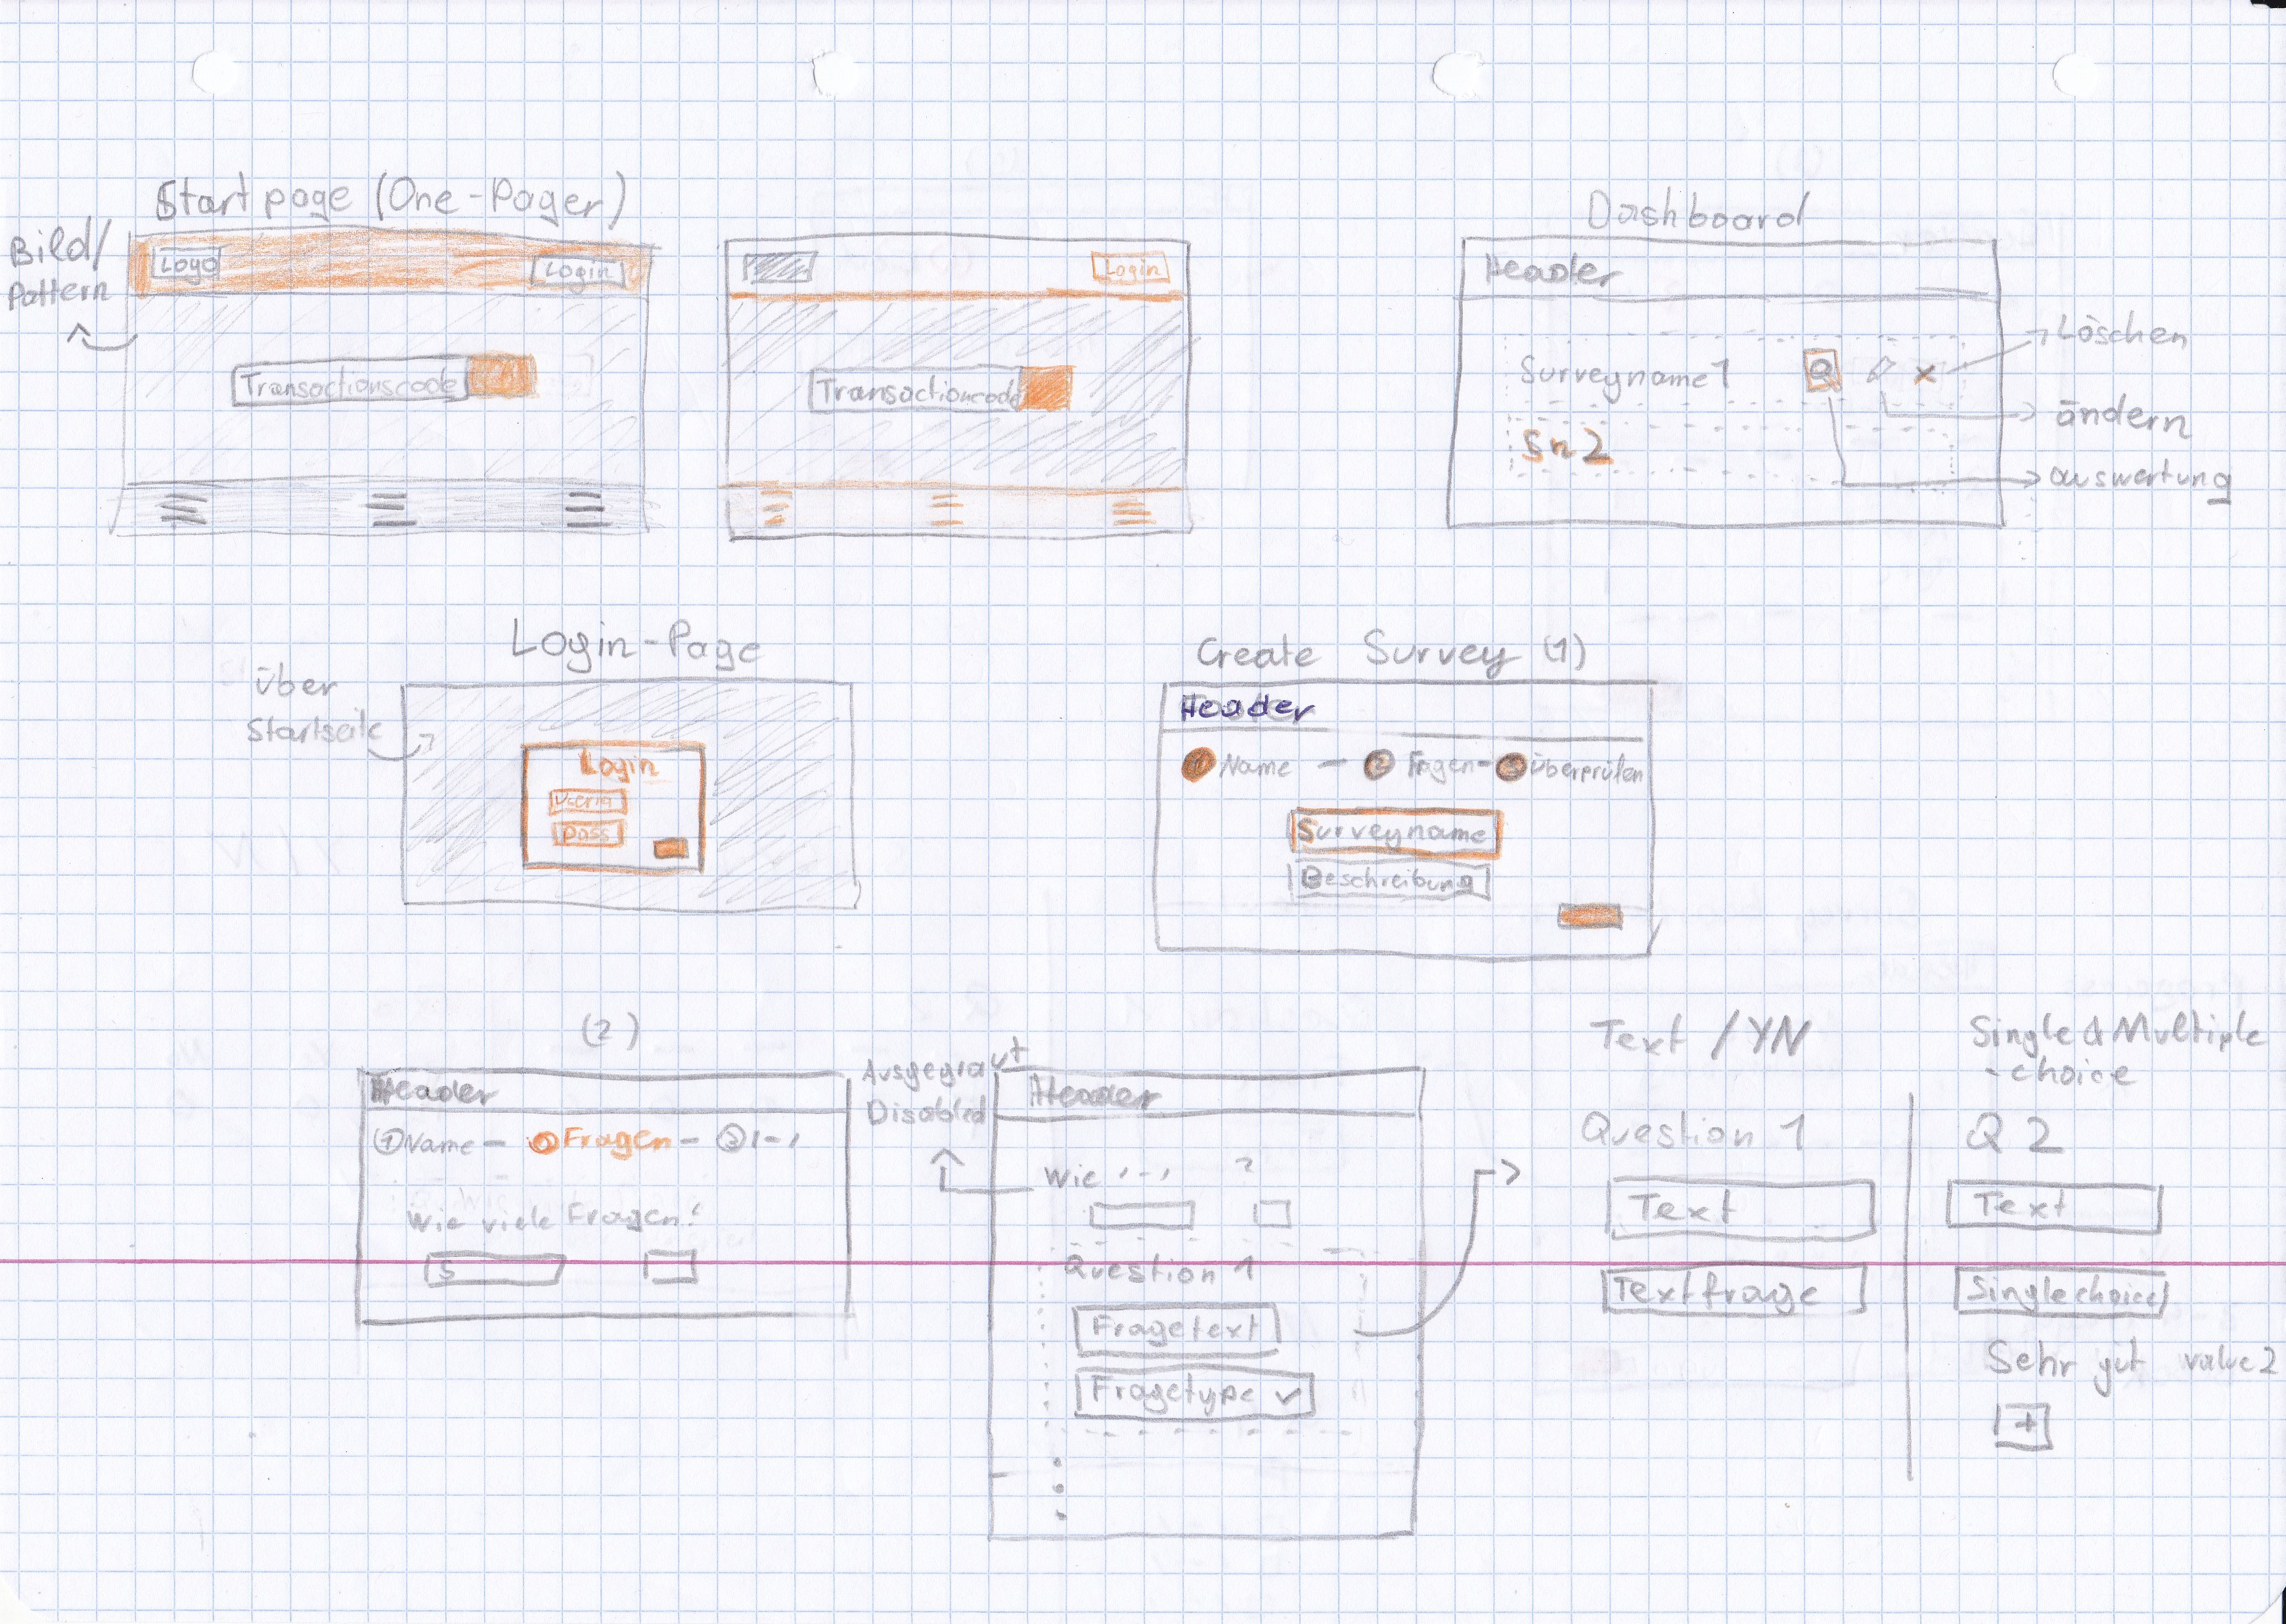
\includegraphics[width=1.0\textwidth]{pics/Handskizze2.jpg}
    \centering
    \caption{Skizze Seite 2}
    \label{fig:skizzen2}
\end{figure}

\newpage

\section{Screendesign Prototyp}
\setauthor{Raffeiner Christine}
Als wichtiger Zwischenschritt zwischen den Skizzen und dem Prototypen wurde ein Moodboard erstellt, dass die grundlegende 
Stimmung der Webseite, wichtige Elemente der zukünftigen Webseite, Schriften und Farben darstellt. Im Moodboard (siehe Abb. \ref{fig:moodboard}) 
wurden die wichtigsten Elemente für die stufenweise Erstellung des Fragebogens, die Fortschrittsanzeige für die 
Beantwortung einer Umfrage und die wichtigsten Funktionen des Dashboard (durch die Icons symbolisiert) erstmals dargestellt.

\begin{figure}[H]
    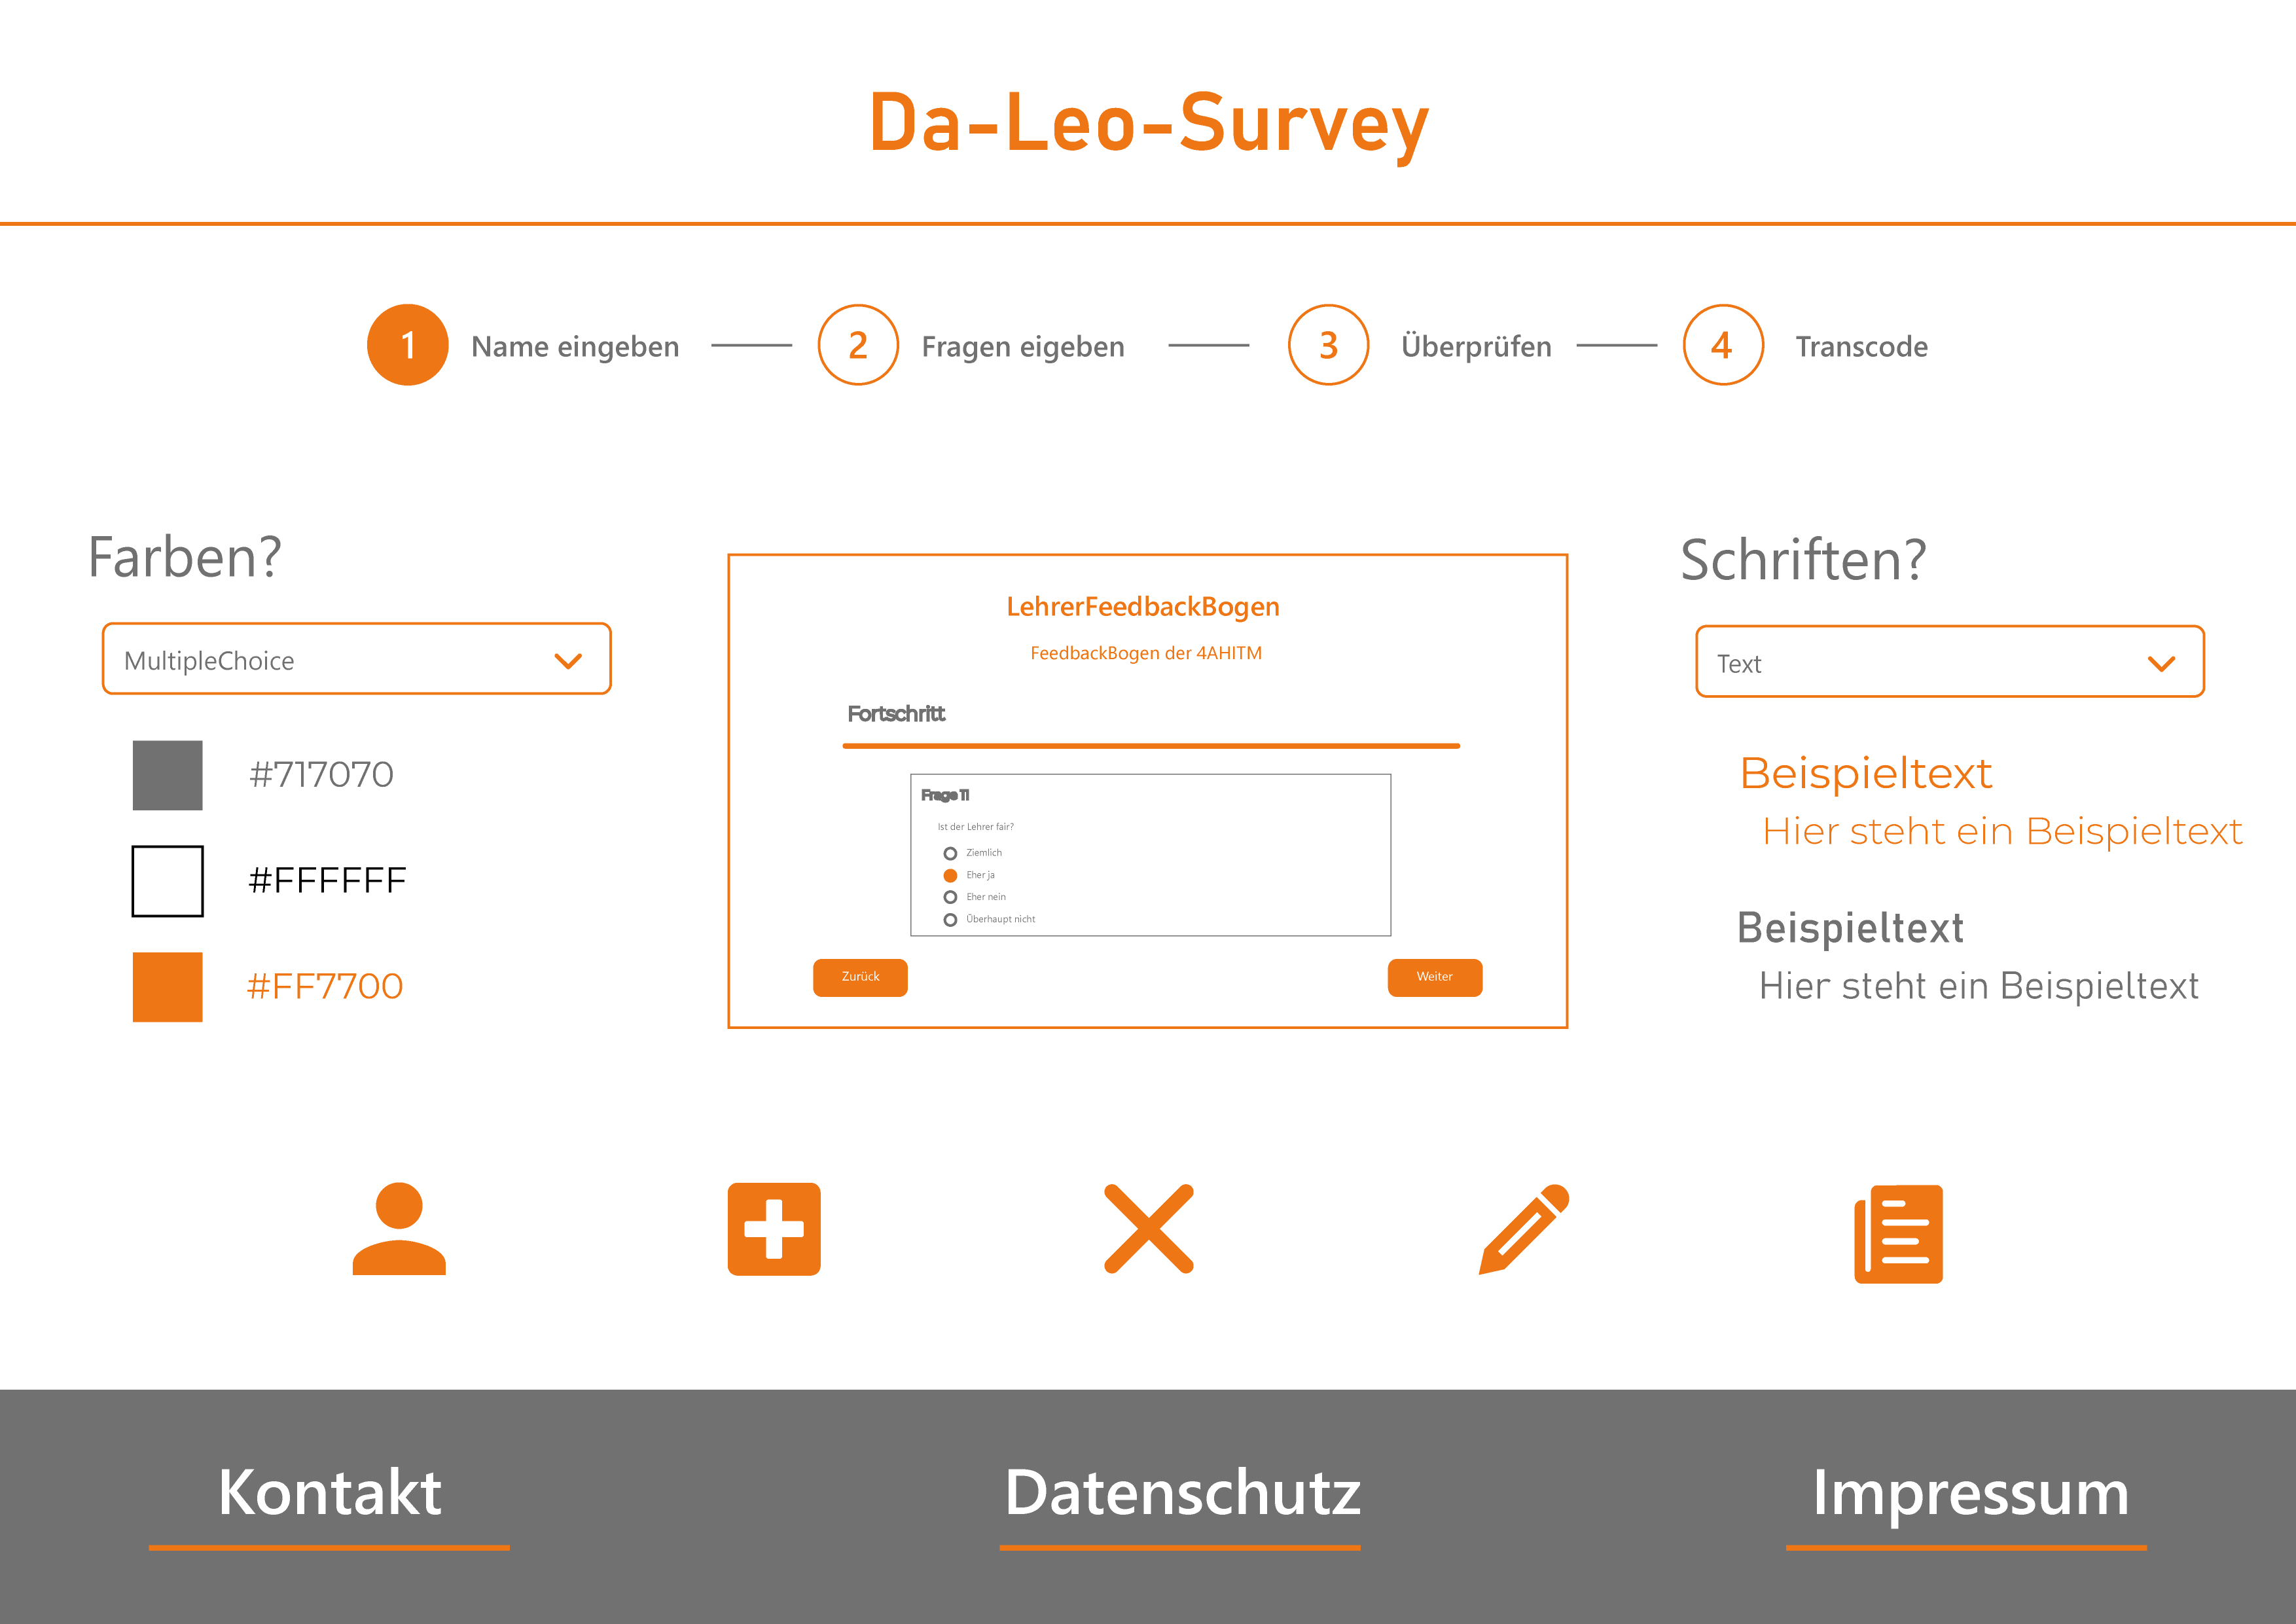
\includegraphics[width=0.8\textwidth]{pics/Moodboard.png}
    \centering
    \caption{Moodboard Leo-Survey}
    \label{fig:moodboard}
\end{figure}

Nach der Erstellung des Moodboards wurden die Skizzen im Programm Adobe XD umgesetzt. 
Es wurde auf das zukünftige Design mit 
Angular Materials Rücksicht genommen und die Elemente möglichst in dem Design von Materials erstellt.

\begin{figure}[H]
    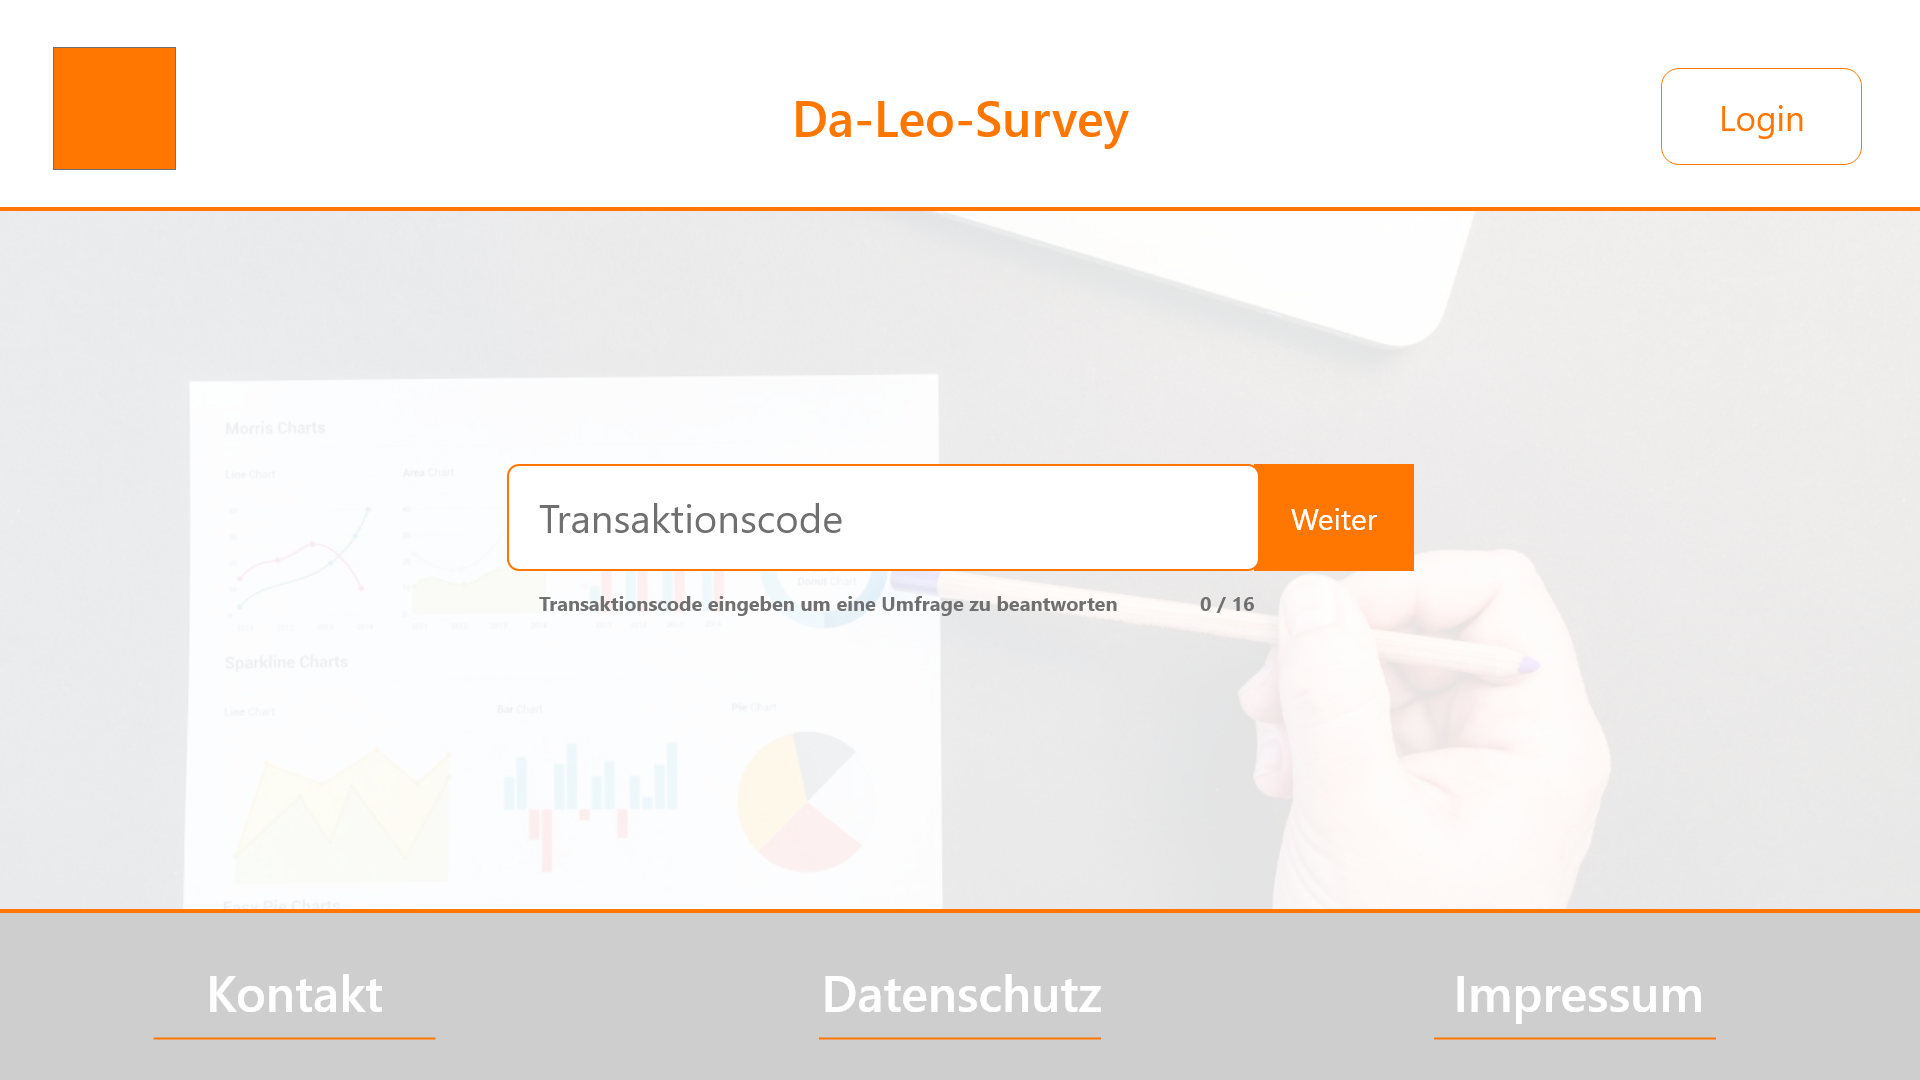
\includegraphics[width=0.8\textwidth]{pics/Startseite.png}
    \centering
    \caption{ScreenDesign Startseite}
    \label{fig:screenDesign2}
\end{figure}

\begin{figure}[H]
    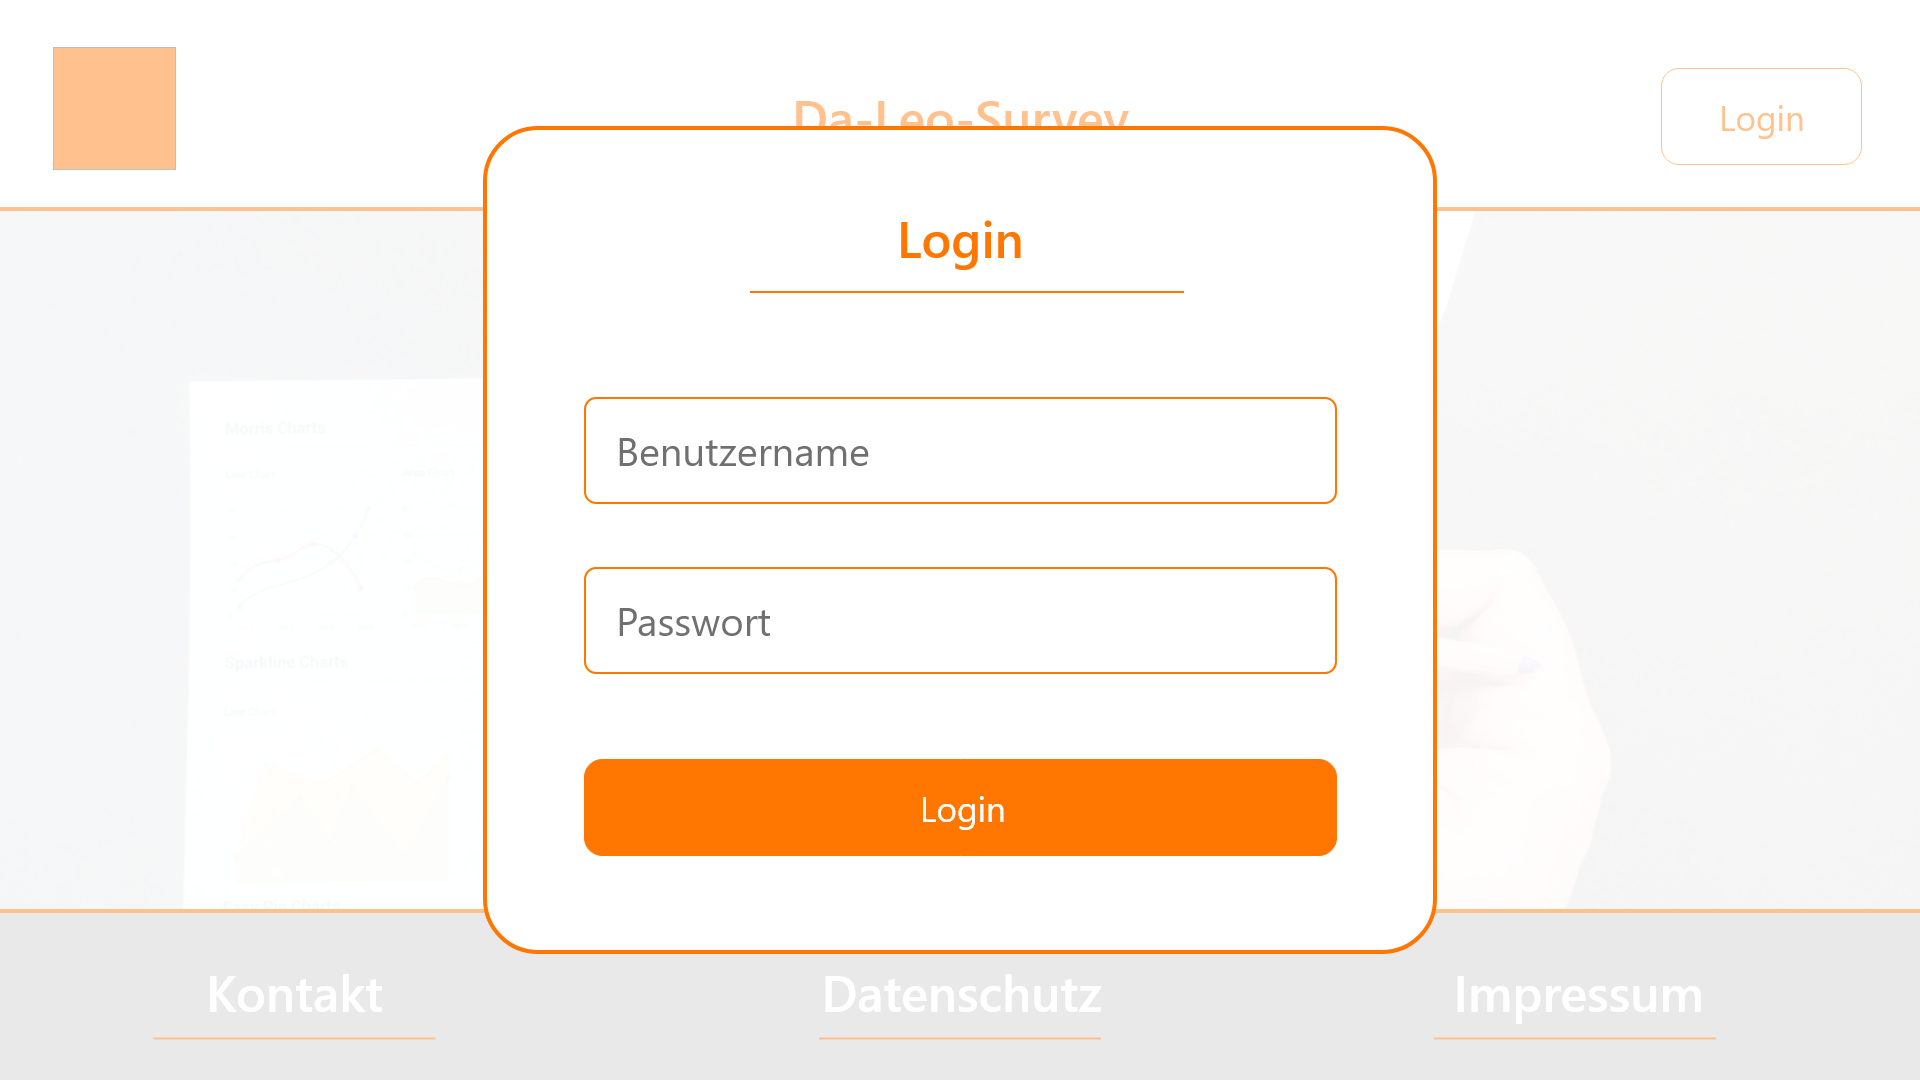
\includegraphics[width=0.8\textwidth]{pics/Login.png}
    \centering
    \caption{ScreenDesign Login}
    \label{fig:screenDesign1}
\end{figure}
    
\begin{figure}[H]
    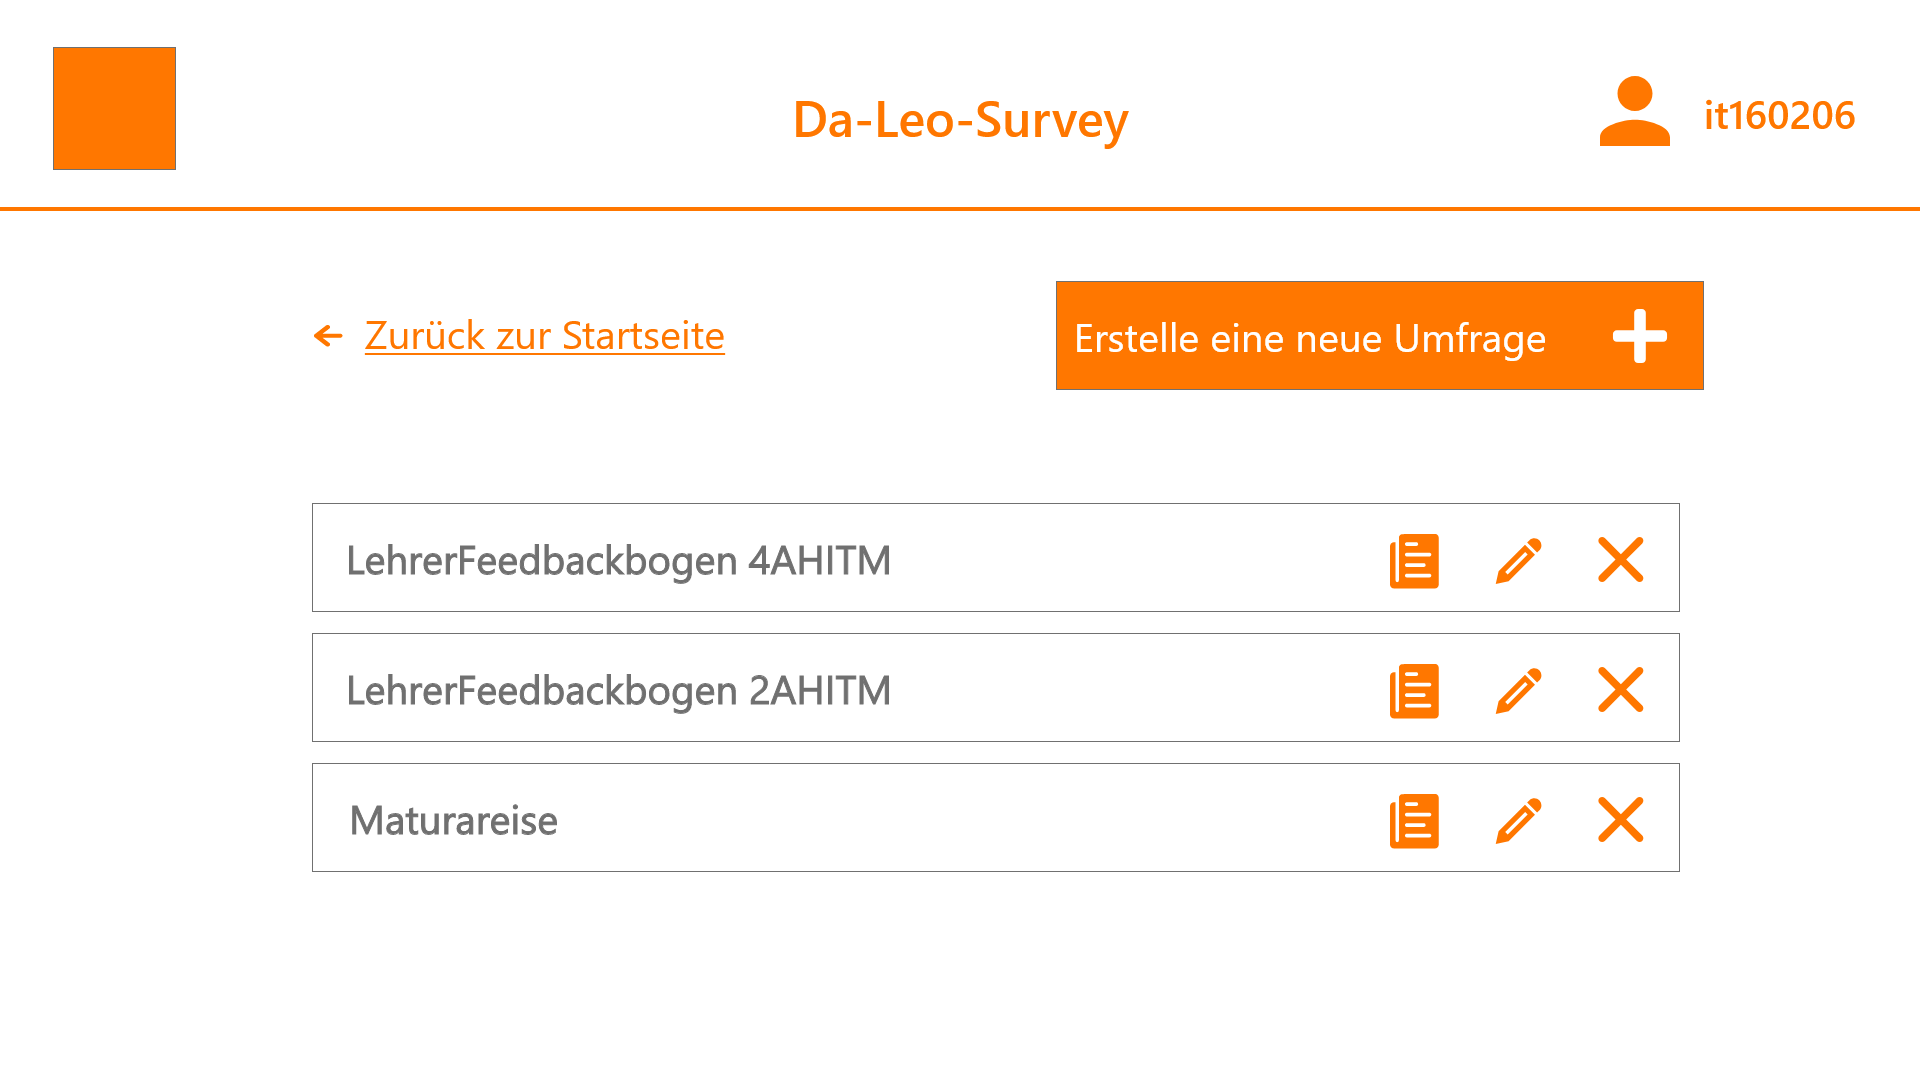
\includegraphics[width=0.8\textwidth]{pics/Dashboard.png}
    \centering
    \caption{ScreenDesign Dashboard}
\end{figure}

\begin{figure}[H]
    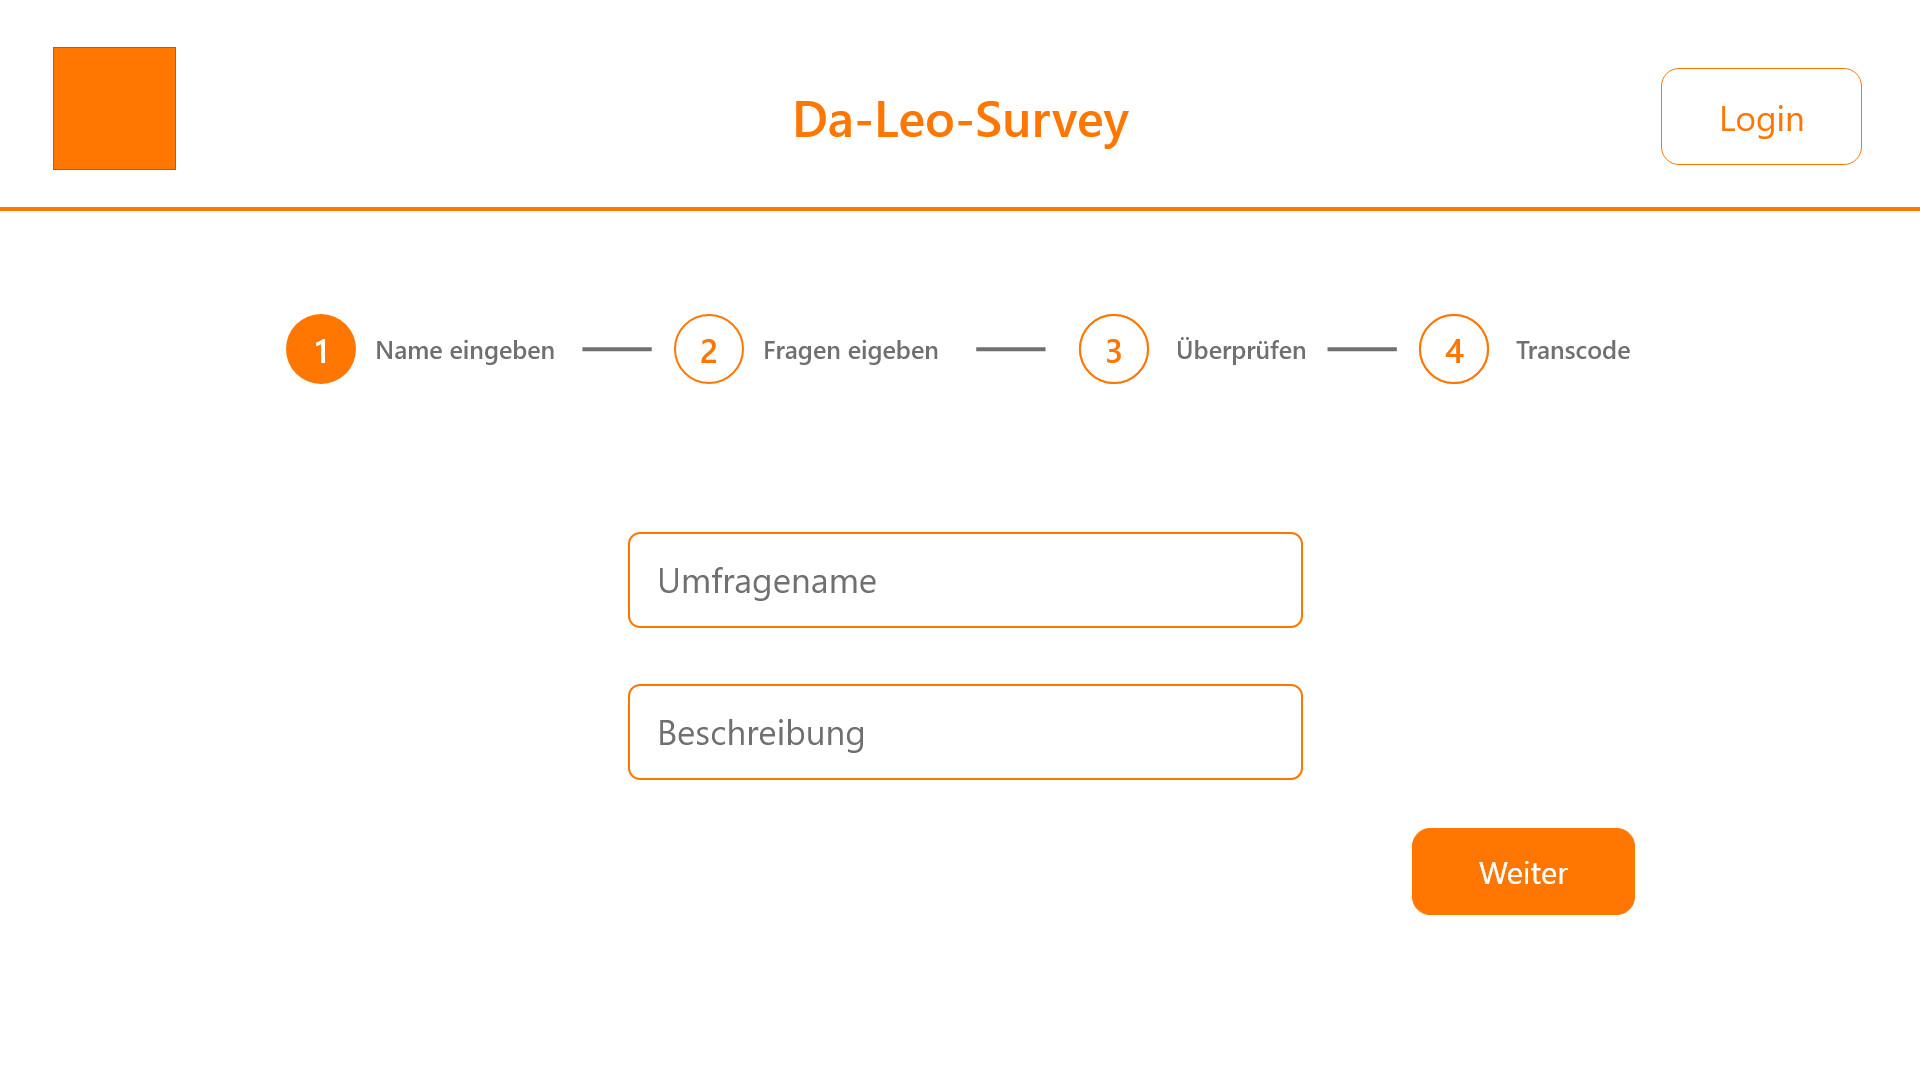
\includegraphics[width=0.8\textwidth]{pics/Erstellen_Umfarage_1.png}
    \centering
    \caption{ScreenDesign Fragebogen erstellen}
\end{figure}

\begin{figure}[H]
    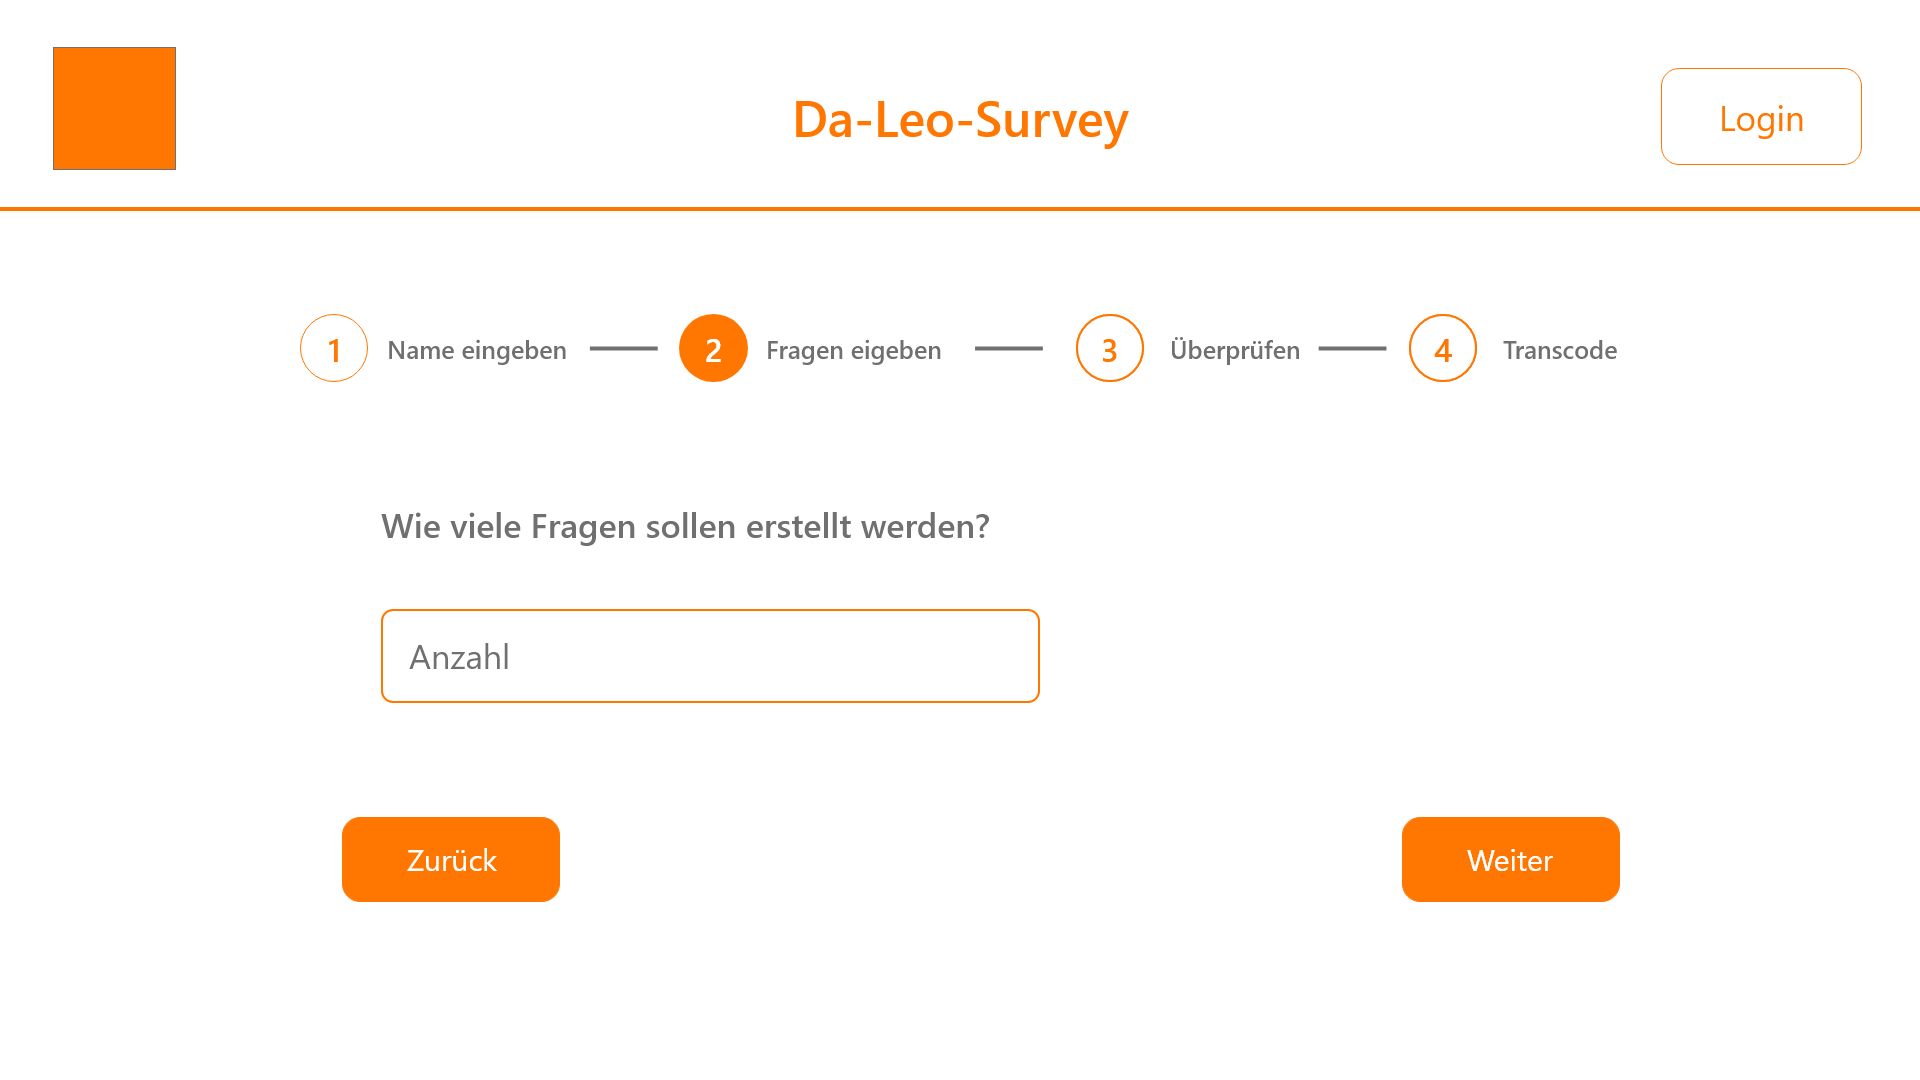
\includegraphics[width=0.8\textwidth]{pics/Erstellen_Umfarage_2.png}
    \centering
    \caption{ScreenDesign Fragebogen erstellen}
\end{figure}

\begin{figure}[H]
    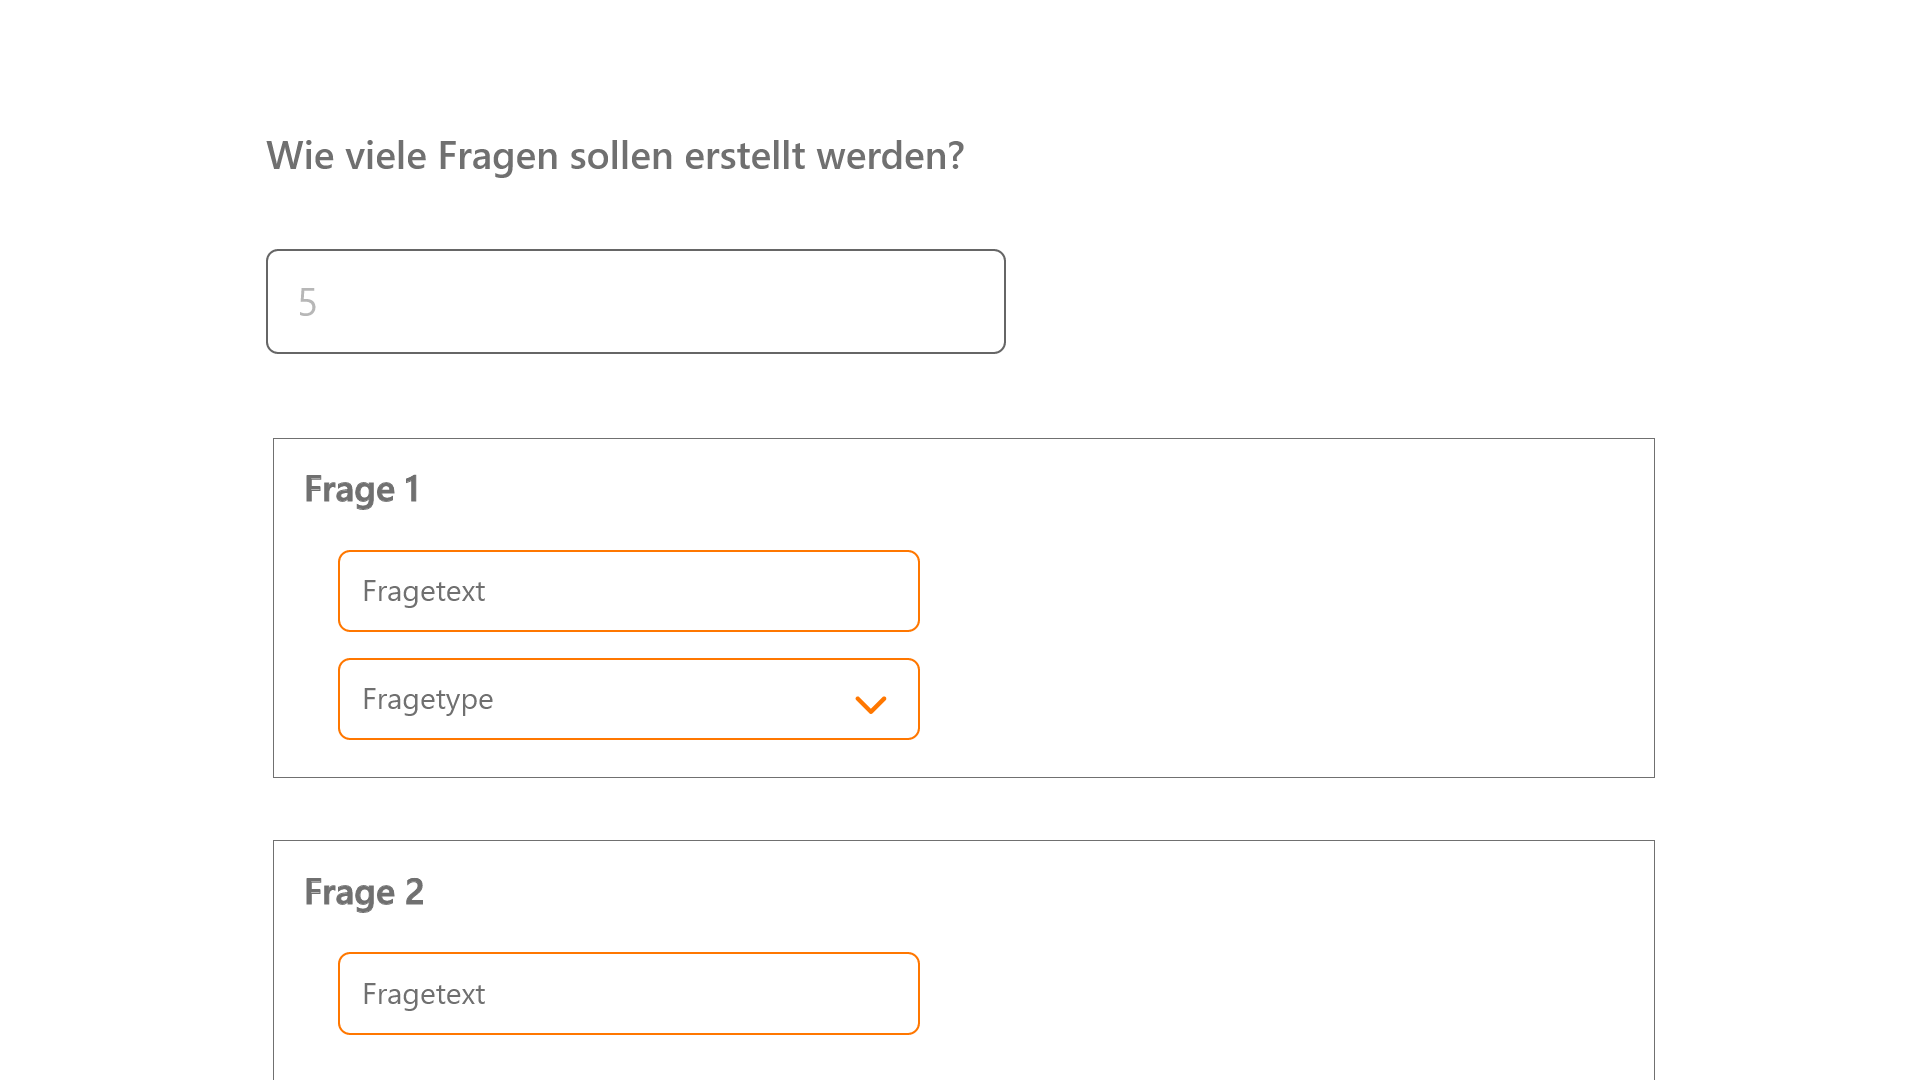
\includegraphics[width=0.4\textwidth]{pics/Erstellen_Umfarage_2_1.png}
    \centering
    \caption{ScreenDesign Fragebogen erstellen}
\end{figure}

\begin{figure}[H]
    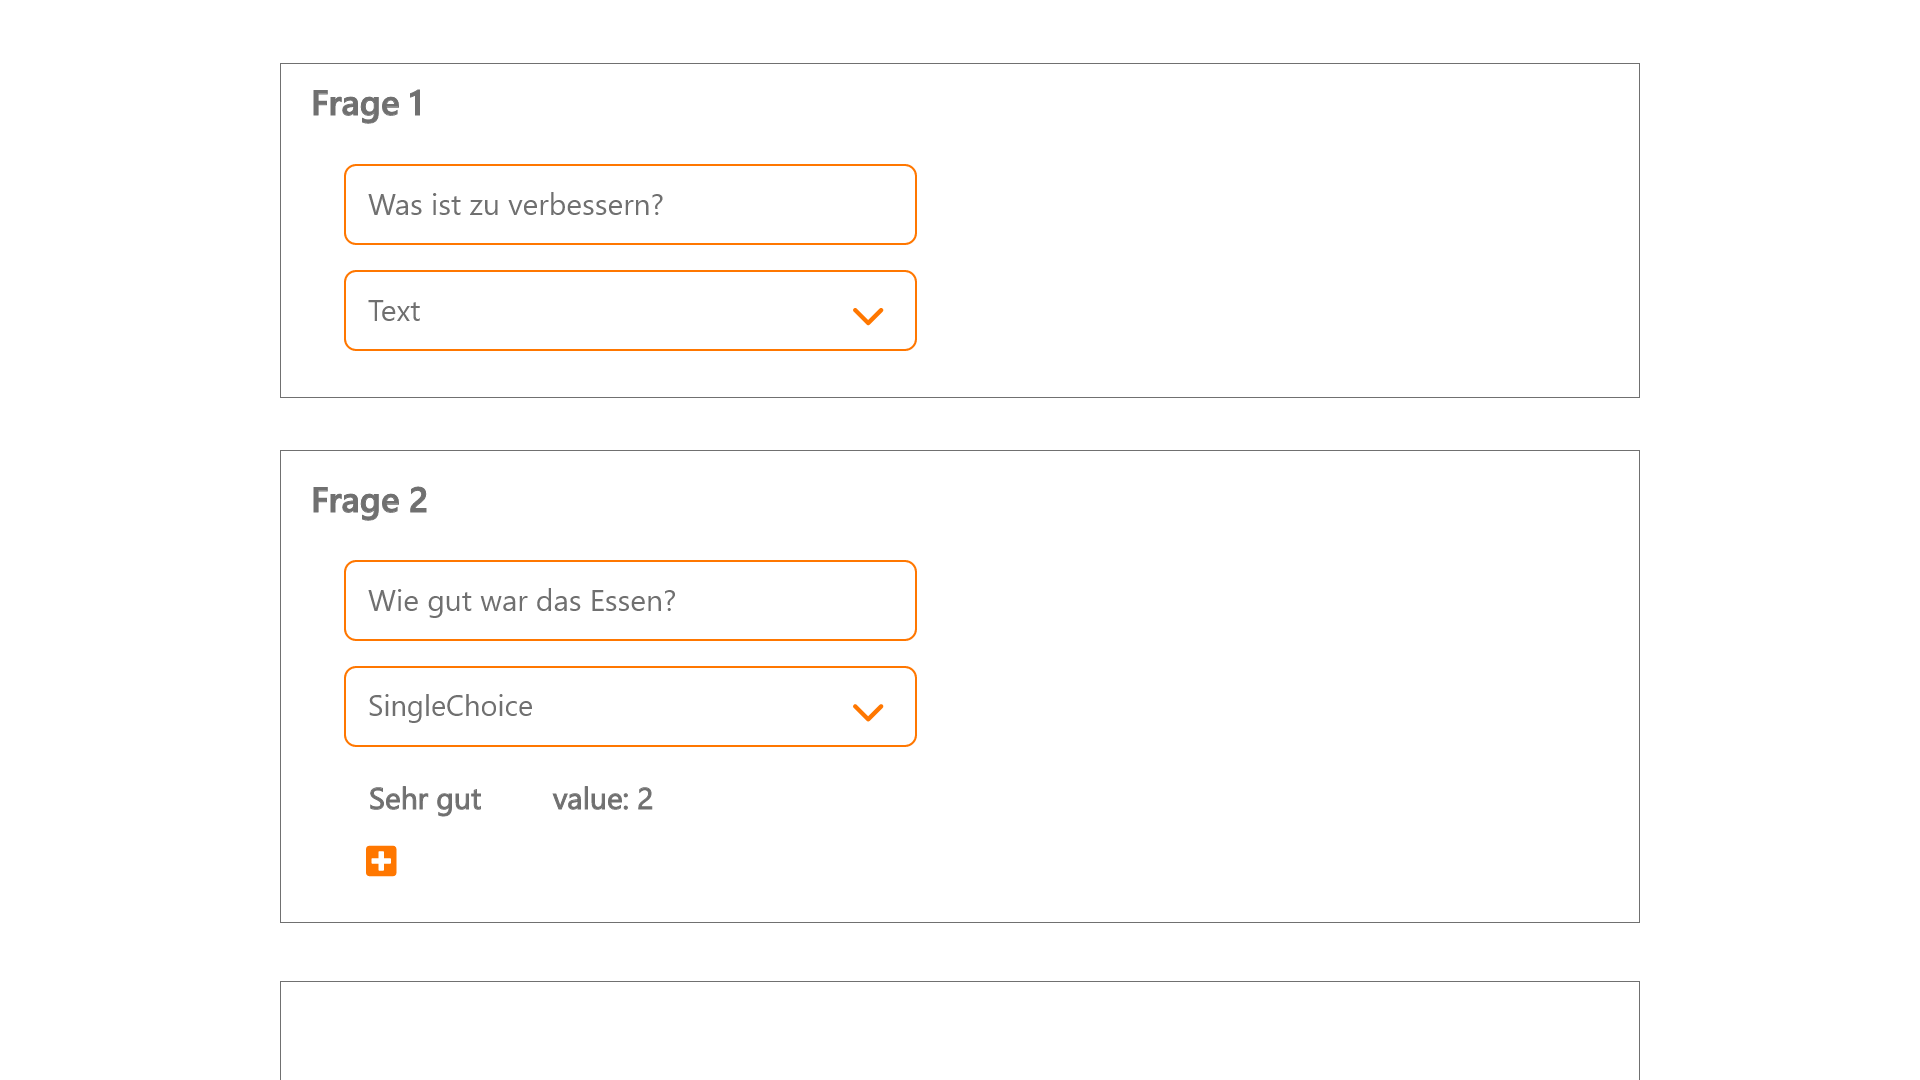
\includegraphics[width=0.4\textwidth]{pics/Erstellen_Umfarage_2_2.png}
    \centering
    \caption{ScreenDesign Fragebogen erstellen}
\end{figure}

\begin{figure}[H]
    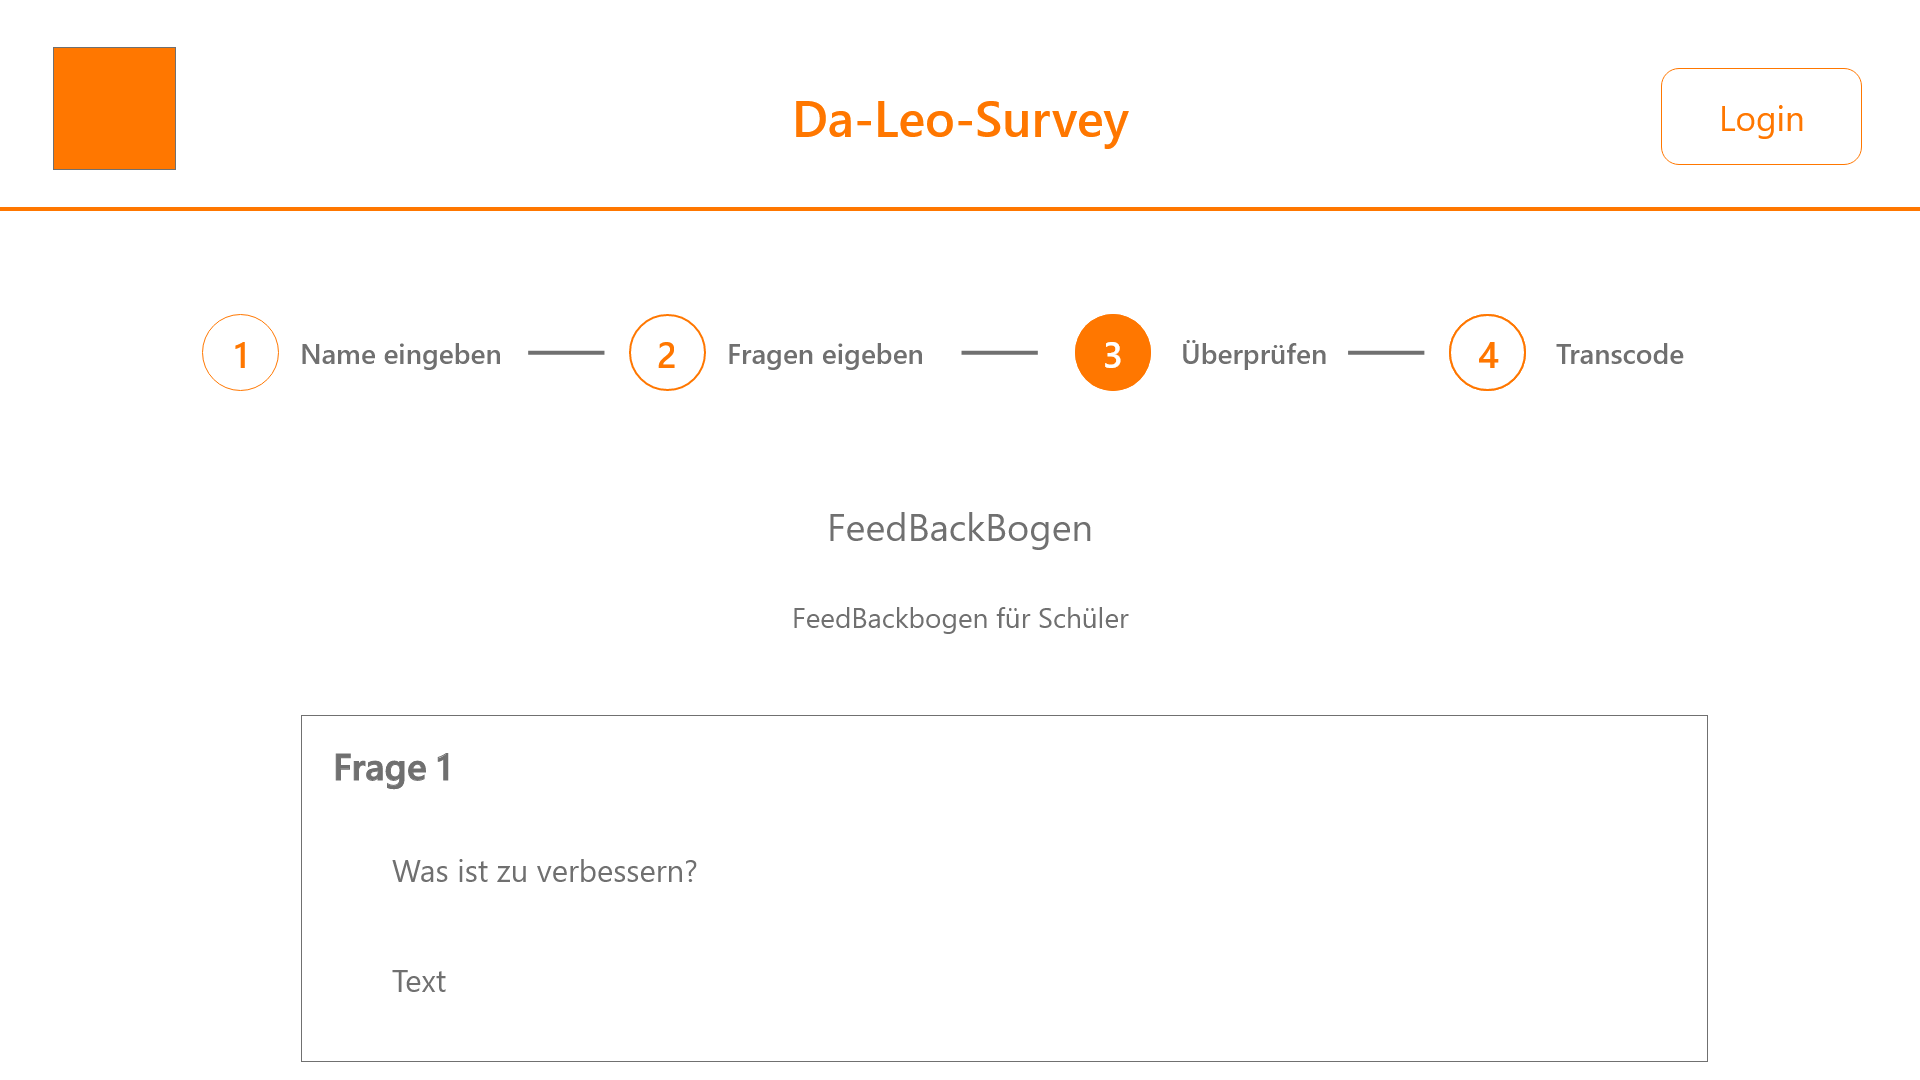
\includegraphics[width=0.8\textwidth]{pics/Erstellen_Umfarage_3.png}
    \centering
    \caption{ScreenDesign Fragebogen erstellen}
\end{figure}

\begin{figure}[H]
    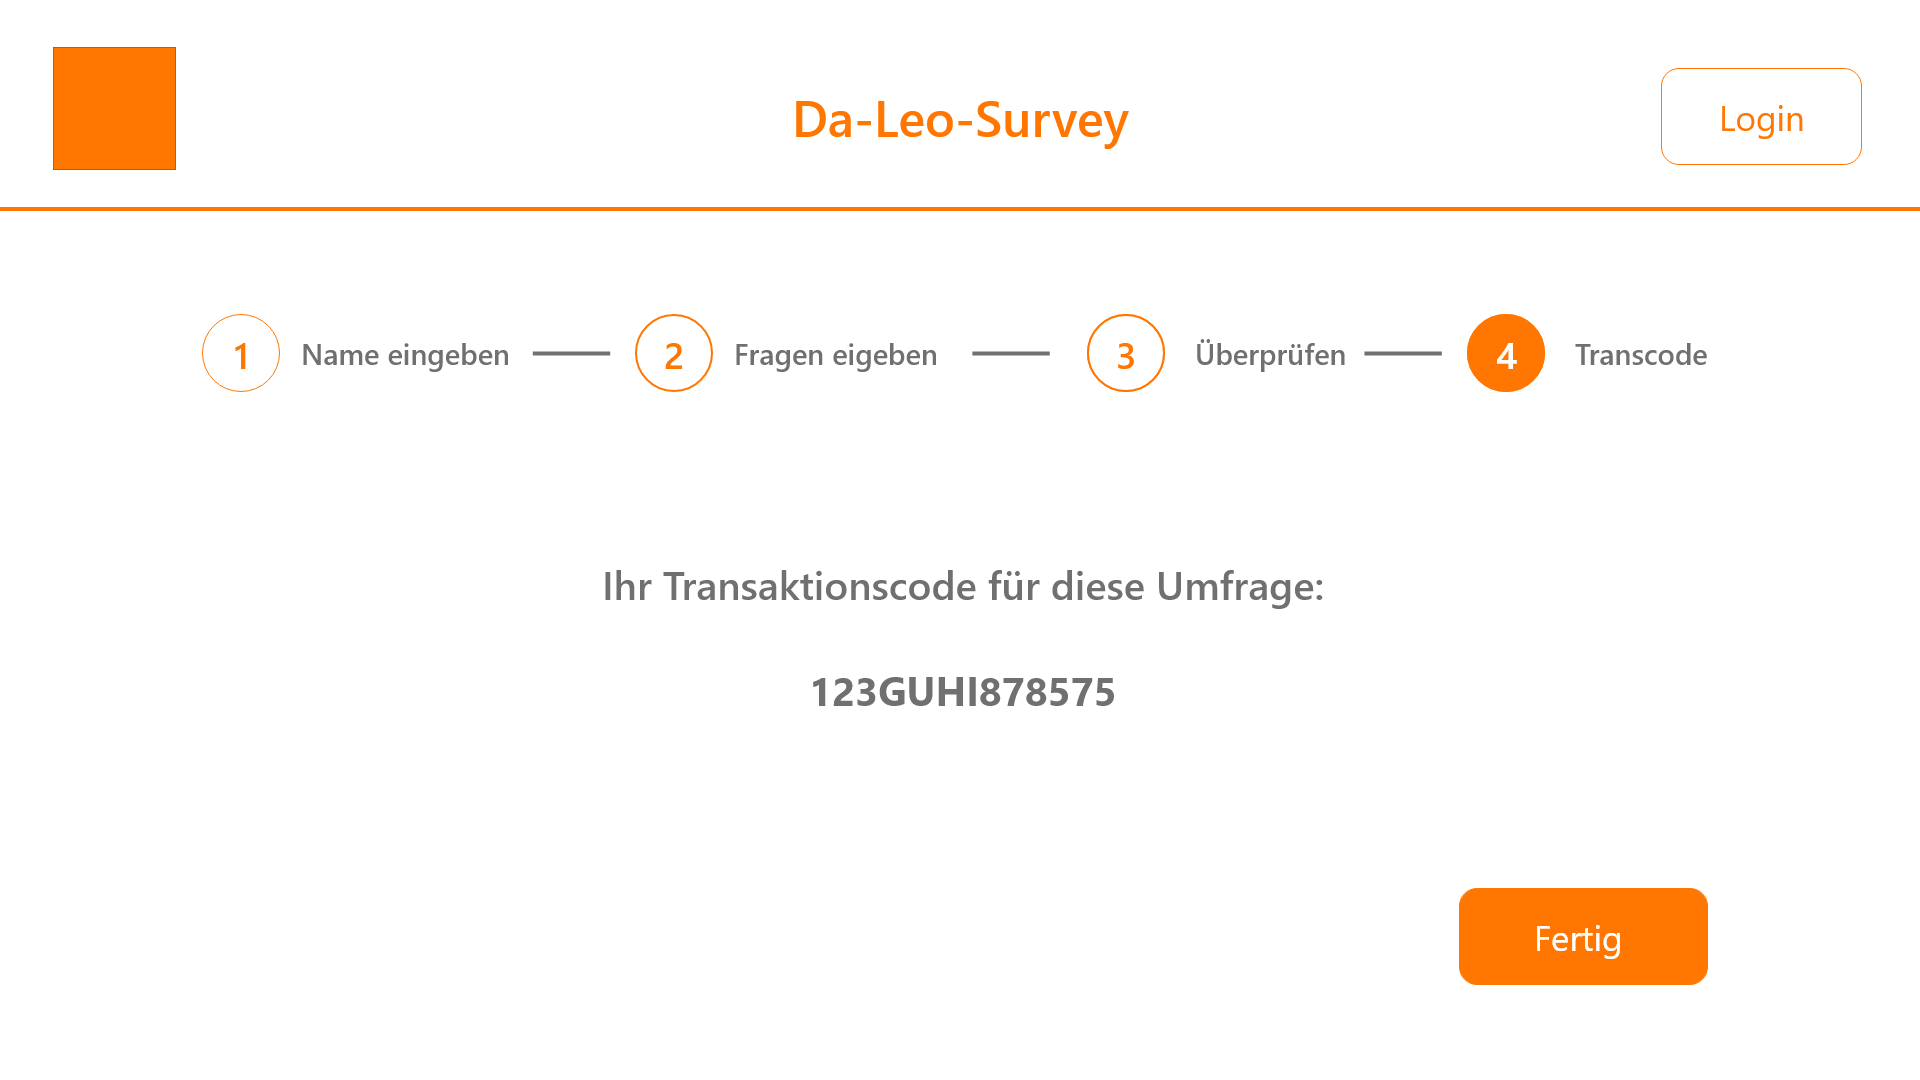
\includegraphics[width=0.8\textwidth]{pics/Erstellen_Umfarage_4.png}
    \centering
    \caption{ScreenDesign Fragebogen erstellen}
\end{figure}

\begin{figure}[H]
    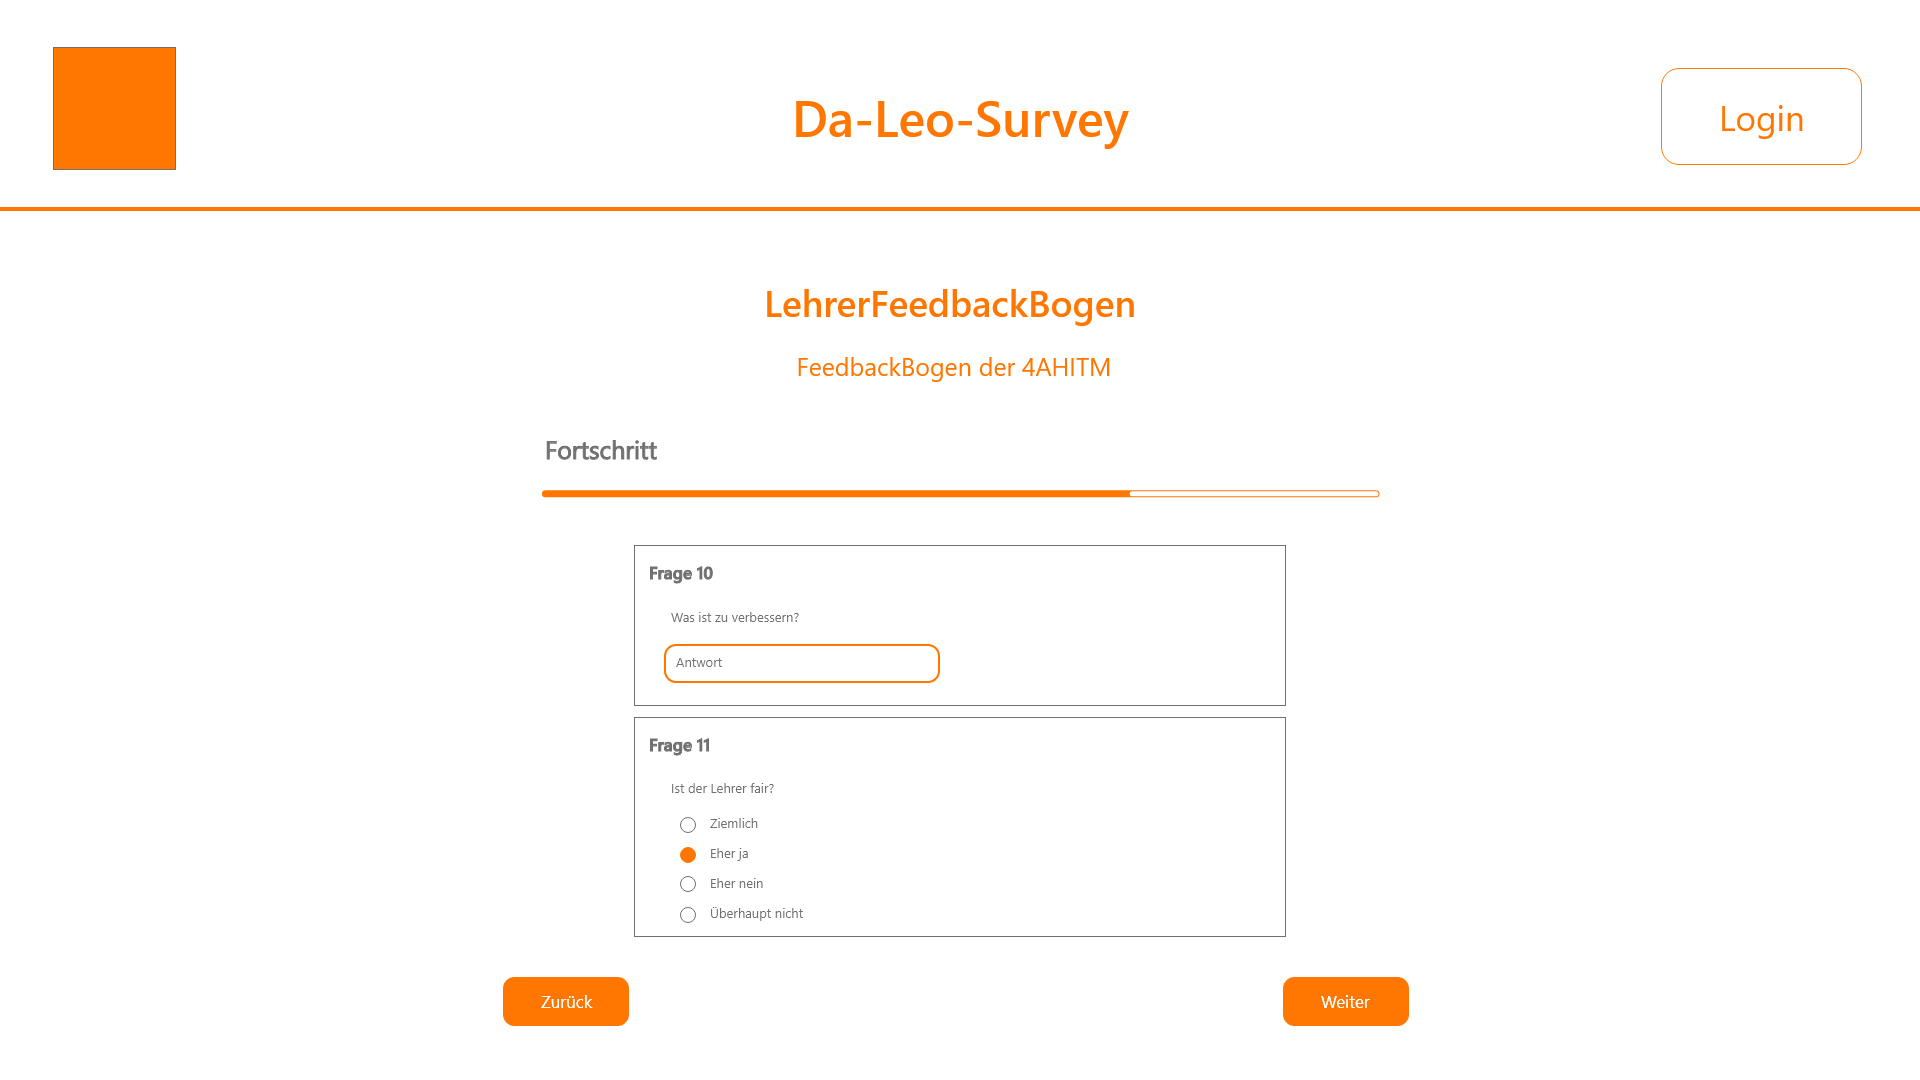
\includegraphics[width=0.8\textwidth]{pics/Fargebogen ausfuellen.png}
    \centering
    \caption{ScreenDesign Fragebogen ausfüllen}
\end{figure}

Die Login-Seite (siehe Abb. \ref{fig:screenDesign1}) wurde im Produktivsystem mit der des Keycloaks ersetzt. Auch andere kleinere Elemente wie der 
Footer auf der Startseite (siehe Abb. \ref{fig:screenDesign2}) wurden in der Engversion abgeändert. Die Endversion befindet sich in Kapitel 
\ref{chapter:ergebnis} auf S. \pageref{chapter:ergebnis}.